%%%%%%%%%%%%%%%%%%%%%%%%%%%%%%%%%%%%%%%%%%%%%%%%%%%%%%%%%%%%%%%%%%%%%%%%%%%%%%%%%%%%%%%%%%%%%%%%%%%%%%%%%%%%%%%%%%%%%%%%

\documentclass[a0paper, portrait, 25pt,
margin=0mm, innermargin=15mm, blockverticalspace=15mm, colspace=15mm, subcolspace=8mm
]{tikzposter}

% font size: 12, 14, 17, 20, 25

% A0 1189x841 2*420.5

%%%%%%%%%%%%%%%%%%%%%%%%%%%%%%%%%%%%%%%%%%%%%%%%%%%%%%%%%%%%%%%%%%%%%%%%%%%%%%%%%%%%%%%%%%%%%%%%%%%%%%%%%%%%%%%%%%%%%%%%<

%%%%%%%%%%%%%%%%%%%%%%%%%%%%%%%%%%%%%%%%%%%%%%%%%%%%%%%%%%%%%%%%%%%%%%%%%%%%%%%%%%%%%%%%%%%%%%%%%%%%%%%%%%%%%%%%%%%%%%%%

%\documentclass[compress,handout]{beamer}
\documentclass[11pt,aspectratio=169,compress,mathserif]{beamer}

% lenovo native resolution is 1600x900 px, 16/9 -> 160mm by 90mm
% 1280x1024 px 5/4.

%%%%%%%%%%%%%%%%%%%%%%%%%%%%%%%%%%%%%%%%%%%%%%%%%%%%%%%%%%%%%%%%%%%%%%%%%%%%%%%%%%%%%%%%%%%%%%%%%%%%%%%%%%%%%%%%%%%%%%%%
%
% Packages
%
%%%%%%%%%%%%%%%%%%%%%%%%%%%%%%%%%%%%%%%%%%%%%%%%%%%%%%%%%%%%%%%%%%%%%%%%%%%%%%%%%%%%%%%%%%%%%%%%%%%%%%%%%%%%%%%%%%%%%%%%

%** Beamer ***************************************

\usepackage{beamerthemefabrice}

\usepackage{pgfpages}
%\pgfpagelayout{resize}[a4paper,border shrink=5mm,landscape]

%**** Tikz ***************************************

\usepackage{transparent}

\usepackage{tikz}
\usetikzlibrary{calc,shapes,backgrounds,arrows}

\usepackage{graphics}

%**** Encoding ***********************************

\usepackage[utf8]{inputenc}
\hypersetup{pdfencoding=auto} % lualatex

%**** Language ***********************************

\usepackage[english]{babel} % -> french

%**** Units and number ***************************

% \usepackage{unite}

%**** Font ***************************************

%\usepackage{fontspec} % spoil circle and textasteriskcentered
%\usepackage{fontawesome} % require lualatex % spoil circle and textasteriskcentered
\usepackage{lmodern} % Postscript layout of CM with T1 coding
%\setsansfont{...}
%? \usepackage{eulervm}
% \usepackage[T1]{fontenc}

%**** Tabular ************************************

%% \usepackage{color}
\usepackage{colortbl}
%% \usepackage{multirow}
%% \usepackage{dcolumn}
%% 
%% \usepackage{cellspace}
%% \setlength{\cellspacebottomlimit}{1pt} 
%% \setlength{\cellspacetoplimit}{1pt} 

%**** Textpos ************************************

\usepackage[absolute,overlay]{textpos} % ,showboxes
\TPGrid{16}{9}

%**** Color **************************************

\usepackage{xcolor}

%*************************************************

% \input{abbreviations}

%\usepackage{alltt}

%%%%%%%%%%%%%%%%%%%%%%%%%%%%%%%%%%%%%%%%%%%%%%%%%%%%%%%%%%%%%%%%%%%%%%%%%%%%%%%%%%%%%%%%%%%%%%%%%%%%%%%%%%%%%%%%%%%%%%%%
%%%
%%% Local Variables: 
%%% mode: latex
%%% TeX-master: "master"
%%% End: 
%%%
%%%%%%%%%%%%%%%%%%%%%%%%%%%%%%%%%%%%%%%%%%%%%%%%%%%%%%%%%%%%%%%%%%%%%%%%%%%%%%%%%%%%%%%%%%%%%%%%%%%%%%%%%%%%%%%%%%%%%%%%

%%%%%%%%%%%%%%%%%%%%%%%%%%%%%%%%%%%%%%%%%%%%%%%%%%%%%%%%%%%%%%%%%%%%%%%%%%%%%%%%%%%%%%%%%%%%%%%%%%%%%%%%%%%%%%%%%%%%%%%%

% Redefinition, symbol included in link:
\let\orighref\href
%\renewcommand{\href}[2]{\orighref{#1}{#2\,\resizebox{!}{1.mm}{\faExternalLink}}} % lualatex
\pgfdeclareimage[height=1mm]{externalLink}{images/external-link-small.png}
\renewcommand{\href}[2]{%
\orighref{#1}{#2\,%
  \begin{tikzpicture}[scale=.1, mystyle/.style={line style=.15pt, line cap=round, line join=round}]
    \draw[mystyle] (1,.4) -- (1,0) -- (0,0) -- (0,1) -- (.7,1);
    \fill (.8,1.2) -- ++(.5,0) -- ++(0,-.5);
    \draw[mystyle] (.6,.4) -- (1.1,1.);
  \end{tikzpicture}%
%\pgfuseimage{externalLink}
}}

%%%%%%%%%%%%%%%%%%%%%%%%%%%%%%%%%%%%%%%%%%%%%%%%%%%%%%%%%%%%%%%%%%%%%%%%%%%%%%%%%%%%%%%%%%%%%%%%%%%%%%%%%%%%%%%%%%%%%%%%

\newcommand{\ptr}{\textasteriskcentered}
\newcommand{\code}[1]{\texttt{#1}}

%%%%%%%%%%%%%%%%%%%%%%%%%%%%%%%%%%%%%%%%%%%%%%%%%%%%%%%%%%%%%%%%%%%%%%%%%%%%%%%%%%%%%%%%%%%%%%%%%%%%%%%%%%%%%%%%%%%%%%%%

\newcommand{\colorR}[1]{{\color{red!80!black}#1}}
\newcommand{\colorG}[1]{{\color{green!80!black}#1}}
\newcommand{\colorB}[1]{{\color{blue!80!black}#1}}
\newcommand{\bgR}{red!20!white}

%%%%%%%%%%%%%%%%%%%%%%%%%%%%%%%%%%%%%%%%%%%%%%%%%%%%%%%%%%%%%%%%%%%%%%%%%%%%%%%%%%%%%%%%%%%%%%%%%%%%%%%%%%%%%%%%%%%%%%%%

\pgfdeclareimage[height=2cm]{FunnyPython}{images/funny-python.png}
\pgfdeclareimage[height=10mm]{FunnyPythonSmall}{images/funny-python.png}
\pgfdeclareimage[height=1cm]{OpenGLLogo}{images/khronos-logos/OpenGL/OpenGL_500.jpg}

%%%%%%%%%%%%%%%%%%%%%%%%%%%%%%%%%%%%%%%%%%%%%%%%%%%%%%%%%%%%%%%%%%%%%%%%%%%%%%%%%%%%%%%%%%%%%%%%%%%%%%%%%%%%%%%%%%%%%%%%
%%%
%%% Local Variables: 
%%% mode: latex
%%% TeX-master: "master"
%%% End: 
%%%
%%%%%%%%%%%%%%%%%%%%%%%%%%%%%%%%%%%%%%%%%%%%%%%%%%%%%%%%%%%%%%%%%%%%%%%%%%%%%%%%%%%%%%%%%%%%%%%%%%%%%%%%%%%%%%%%%%%%%%%%


%%%%%%%%%%%%%%%%%%%%%%%%%%%%%%%%%%%%%%%%%%%%%%%%%%%%%%%%%%%%%%%%%%%%%%%%%%%%%%%%%%%%%%%%%%%%%%%%%%%%%%%%%%%%%%%%%%%%%%%%<

\title{Une interface expérimentale pour lier OpenGL à Python}
\author{Fabrice~Salvaire}
% \institute{}
\pgfdeclareimage[height=10cm]{FunnyPython}{images/funny-python.png}
\pgfdeclareimage[height=10cm]{OpenGLLogo}{images/OpenGL_1500.png}
\titlegraphic{\pgfuseimage{OpenGLLogo}\pgfuseimage{FunnyPython}}

\newcommand{\emailOrange}{fabrice.salvaire@orange.fr}
\newcommand{\homePageOrange}{\url{http://fabrice-salvaire.pagesperso-orange.fr}}
% \newcommand{\homePageGithub}{\url{http://fabricesalvaire.github.io}}
\newcommand{\githubRepositories}{\url{http://github.com/FabriceSalvaire}}

%%%%%%%%%%%%%%%%%%%%%%%%%%%%%%%%%%%%%%%%%%%%%%%%%%%%%%%%%%%%%%%%%%%%%%%%%%%%%%%%%%%%%%%%%%%%%%%%%%%%%%%%%%%%%%%%%%%%%%%%
%
% Settings
%
%%%%%%%%%%%%%%%%%%%%%%%%%%%%%%%%%%%%%%%%%%%%%%%%%%%%%%%%%%%%%%%%%%%%%%%%%%%%%%%%%%%%%%%%%%%%%%%%%%%%%%%%%%%%%%%%%%%%%%%%

% Beamer %%%%%%%%%%%%%%%%%%%%%%%%%%%%%%%%%%%%%%%%%%%%%%%%%%%%%%%%%%%%%%%%%%%%%%%%%%%%%%%%%%%%%%%%%%%%%%%%%%%%%%%%%%%%%%%

\mode<presentation>
{
  \usetheme{fabrice}
  % \usetheme{Madrid}
  % \usetheme{Warsaw}

  \setbeamersize{text margin left=5mm}
  \setbeamersize{text margin right=5mm}

  \setbeamertemplate{navigation symbols}{}
  % \setbeamertemplate{blocks}[rounded][shadow=false] % done
  \setbeamertemplate{itemize items}[circle]
  \setbeamertemplate{enumerate items}[circle]

  % \setbeamercovered{transparent}

  % \setbeamertemplate{background}[grid][step=1cm]
}

\setbeameroption{hide notes}
% \setbeameroption{show notes}
% \setbeameroption{show notes on second screen}
% \setbeameroption{show only notes}

% Comment this, if you do not want the table of contents to pop up at the beginning of each subsection:
% \AtBeginSubsection[]
% {
%  \begin{frame}<beamer>
%    \frametitle{Outline}
%    \tableofcontents[currentsection,currentsubsection]
%  \end{frame}
% }

% If you wish to uncover everything in a step-wise fashion, uncomment the following command: 
% \beamerdefaultoverlayspecification{<+->}

%%%%%%%%%%%%%%%%%%%%%%%%%%%%%%%%%%%%%%%%%%%%%%%%%%%%%%%%%%%%%%%%%%%%%%%%%%%%%%%%%%%%%%%%%%%%%%%%%%%%%%%%%%%%%%%%%%%%%%%%
%%%
%%% Local Variables: 
%%% mode: latex
%%% TeX-master: "master"
%%% End: 
%%%
%%%%%%%%%%%%%%%%%%%%%%%%%%%%%%%%%%%%%%%%%%%%%%%%%%%%%%%%%%%%%%%%%%%%%%%%%%%%%%%%%%%%%%%%%%%%%%%%%%%%%%%%%%%%%%%%%%%%%%%%


%%%%%%%%%%%%%%%%%%%%%%%%%%%%%%%%%%%%%%%%%%%%%%%%%%%%%%%%%%%%%%%%%%%%%%%%%%%%%%%%%%%%%%%%%%%%%%%%%%%%%%%%%%%%%%%%%%%%%%%%

\begin{document}
%
\maketitle
%
\begin{columns}
%%%%%%%%%%%%%%%%%%%%%%%%%%%%%%%%%%%%%%%%%%%%%%%%%%%%%%%%%%%%%%%%%%%%%%%%%%%%%%%%
% First column
\column{.5}

\block{OpenGL~: C'est quoi?}{
  \begin{minipage}{.2\linewidth}
    \begin{center}
      
\includegraphics[width=.8\textwidth]{images/khronos-logos/OpenGL/OpenGL_500.jpg} \\
      
\includegraphics[width=.8\textwidth]{images/khronos-logos/OpenGL_ES/OpenGL-ES_500.jpg} \\
      
\includegraphics[width=.8\textwidth]{images/khronos-logos/WebGL/WebGL_500.jpg} \\
      
\includegraphics[width=.8\textwidth]{images/khronos-logos/Khronos_Group/Khronos_Group_500.jpg}
    \end{center}
  \end{minipage}
  \begin{minipage}{.8\linewidth}
    \begin{itemize}
    \item Un standard \textbf{ouvert} piloté par le groupe Khronos
    \item La seule API \textbf{cross-platforme} et \textbf{cross-vendor} % cross / multi
    \item L'API de facto de GNU/Linux et d'Android
    \item Une API orientée desktop (OpenGL) et embarqué (OpenGL ES)
    \item et aussi orientée web (WebGL)
    \end{itemize}
  \end{minipage}
}

\block{XML API Registry}{
  % \begin{tikzpicture}[remember picture, overlay, mystyle/.style={fill=red!20, opacity=1.}] % run twice
  %   \fill[mystyle] ($(current page.south west) + (2.4,3.3)$) rectangle +(3.2,.5);
  %   \node [mystyle, rectangle callout, callout relative pointer={(-3.5,-.5)}]
  %   at ($(current page.south west) + (10,4.5)$) {la taille est indiqué};
  % \end{tikzpicture}
  Fichier XML définissant~:
  % https://www.opengl.org/registry
  \begin{itemize}
    \item les constantes
    \item les fonctions et leurs prototypes \\[.5em]
      \footnotesize{\code{%
void glClearBufferData (GLenum target, GLenum internalformat, GLenum format, GLenum type, const void * data) \\[1em]
<command> \\
% \hspace{1cm}
\rule{2em}{0pt} <proto>void <name>glClearBufferData</name></proto> \\
\rule{2em}{0pt} \ldots \\
\rule{2em}{0pt} <param><ptype>GLenum</ptype> <name>format</name></param> \\
\rule{2em}{0pt} <param><ptype>GLenum</ptype> <name>type</name></param> \\
\rule{2em}{0pt} <param len="COMPSIZE(format,type)">const void *<name>data</name></param> \\
</command>
}}
% \begin{Verbatim}[commandchars=\\\{\}]
%  void glClearBufferData (GLenum target, GLenum internalformat, GLenum format, GLenum type, const void * data)
%
% <command>
%     <proto>void <name>glClearBufferData</name></proto>
%     ...
%     <param><ptype>GLenum</ptype> <name>format</name></param>
%     <param><ptype>GLenum</ptype> <name>type</name></param>
%     <param len="COMPSIZE(format,type)">const void *<name>data</name></param>
% </command>
% \end{Verbatim}}
    \item les extensions
    \item les \textbf{versions} et leurs \textbf{profiles}
  \end{itemize}
  \centerline{\colorR{$\longrightarrow$ Apporte des informations essentielles par rapport au fichier d'en-tête}}
  \note{
    \begin{enumerate}
    \item 
    \end{enumerate}
  }
}

% \block{Architecture}{
%   \begin{center}
%   \begin{tikzpicture}[]
%     %\draw[help lines] (-15,-20) grid (15,20);
%     \node at (0,0) {\includegraphics[width=30cm]{images/tree.pdf}};
%     \node at (-12,5) {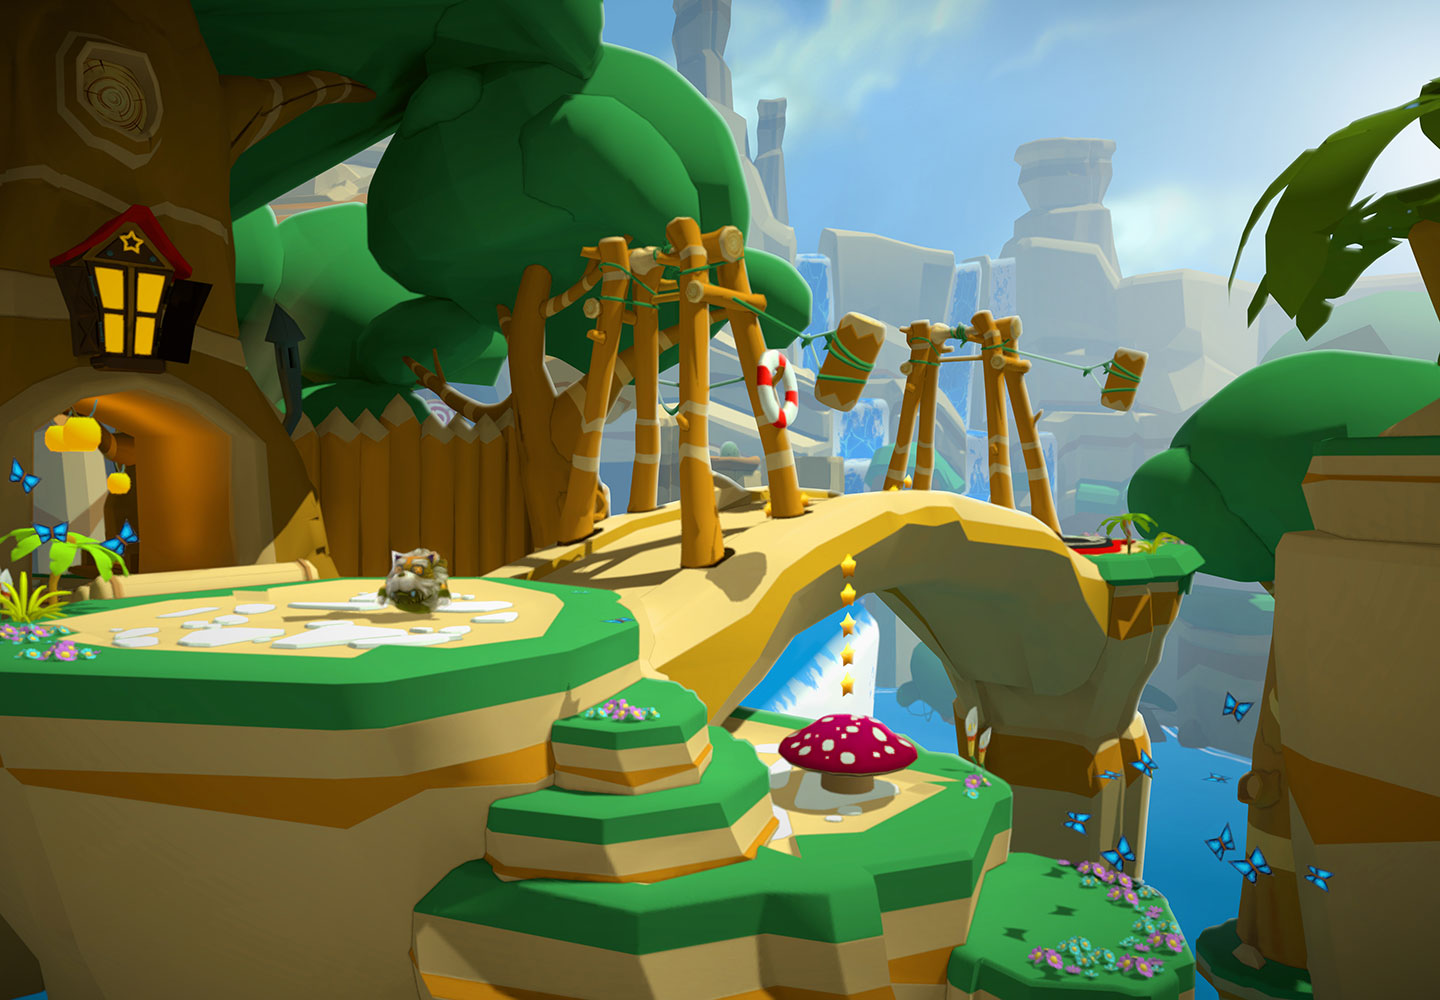
\includegraphics[width=10cm]{images/game.jpg}};
%     \node at (-8,15) {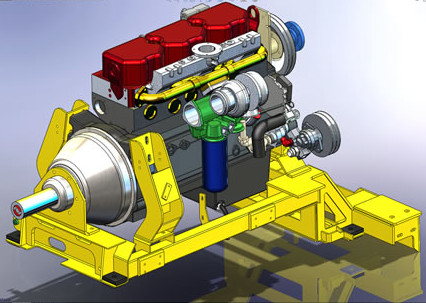
\includegraphics[width=10cm]{images/solidworks.jpg}};
%     \node at (1,15) {
\includegraphics[height=10cm]{images/touchwiz.jpg}};
%     \node at (8,10) {
\includegraphics[width=10cm]{images/tiger.png}};
%     \node at (12,2) {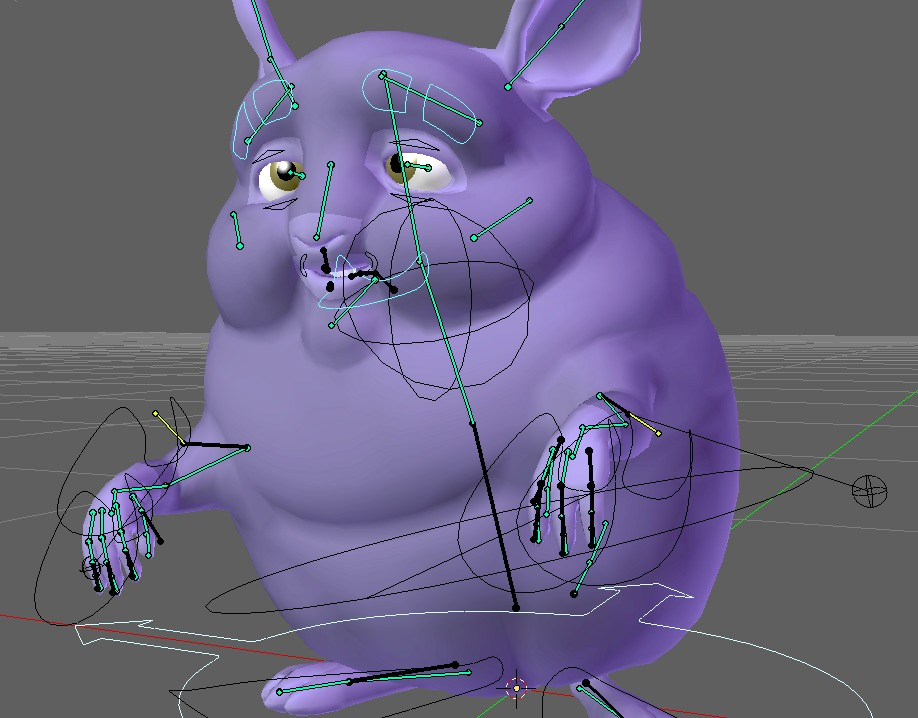
\includegraphics[width=8cm]{images/blender.jpg}};
%     \node at (-13,-6) {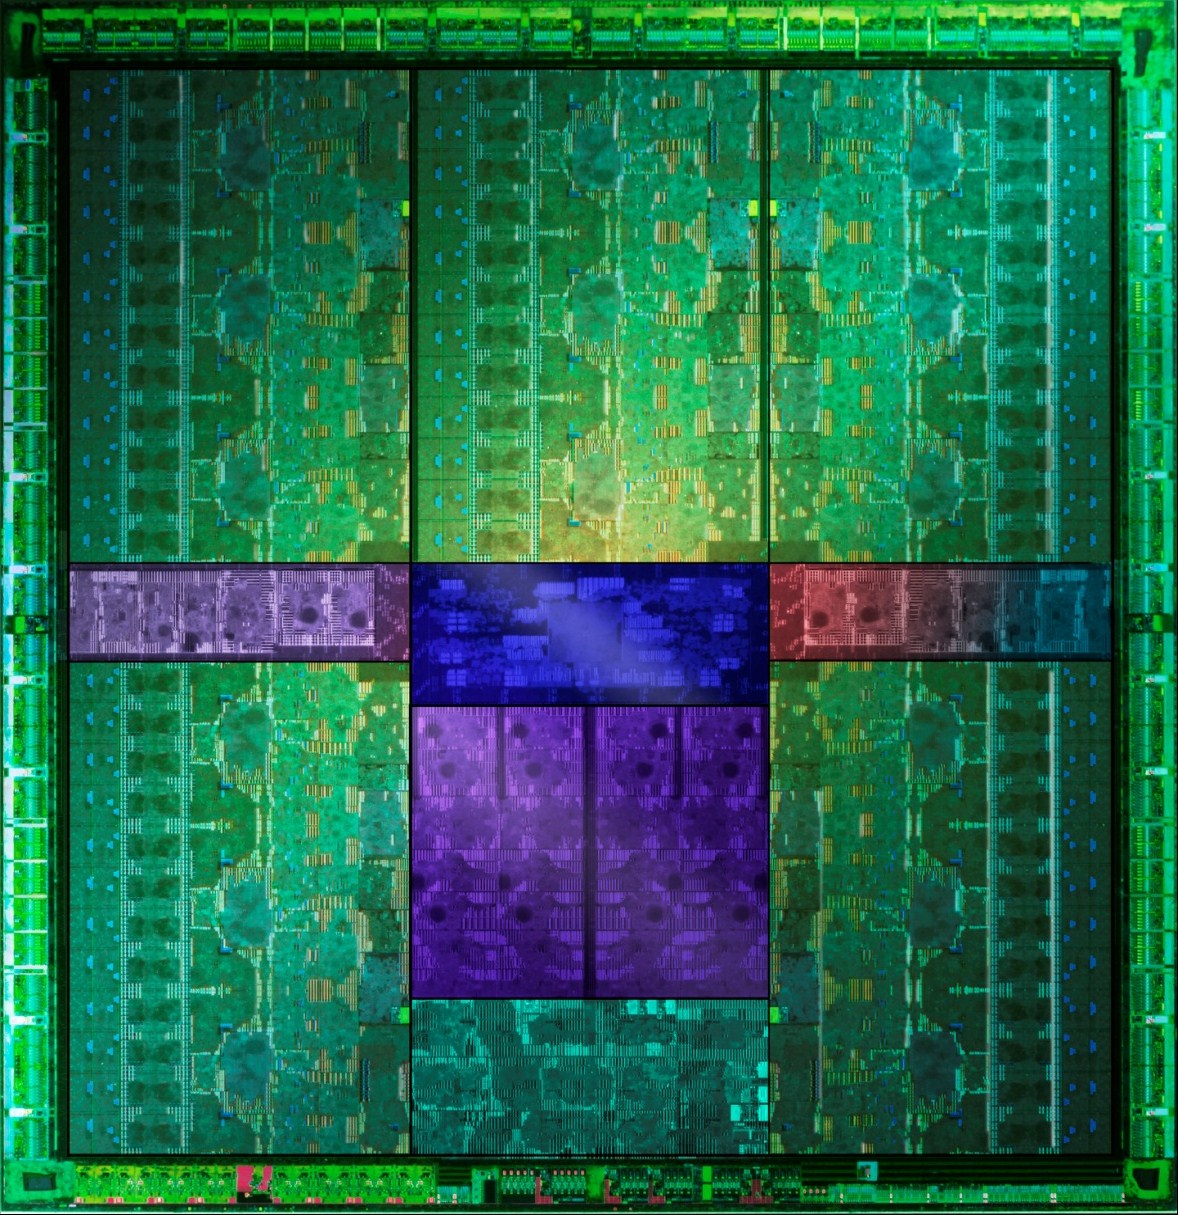
\includegraphics[width=4cm]{images/nvidia-kepler-die.jpg}};
%     \begin{scope}[xshift=-3cm, yshift=-12cm,
%       base/.style={rectangle, minimum width=10em, minimum height=2em, draw=white, line width=2pt,
%         anchor=south west},
%       double/.style={base, minimum height=4em},
%       small/.style={base, minimum width=4em}]
%       % \draw [help lines] grid(3,2);
%       \node[base, fill=green!20] at (0,0) {XML Registry};
%       \node[base, fill=red!20] at (0,2em) {GL API};
%       \node[double, fill=blue!20] at (0,4em) {Wrapper};
%       \node[small, fill=green!20] at (-4em,4em) {ctypes};
%       \node[small, fill=red!20] at (-4em,6em) {cffi};
%       \node[double, minimum width=4em, fill=blue!20] at (-8em,4em) {GL};
%       \node[base, fill=green!20] at (0,8em) {High Level API};
%     \end{scope}
%     \end{tikzpicture}
%   \end{center}
% }

\block{Architecture}{
  \begin{center}
  \begin{tikzpicture}[]
    %\draw[help lines] (-15,-20) grid (15,20);
    \node at (0,0) {\includegraphics[width=30cm]{../images/Adansonia_grandidieri04.jpg}};
    \node at (-10,4) {
\includegraphics[width=6cm]{images/tiger.png}};
    \node at (-8,12) {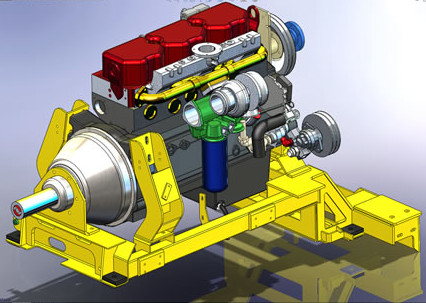
\includegraphics[width=6cm]{images/solidworks.jpg}};
    \node at (1,15) {
\includegraphics[height=6cm]{images/touchwiz.jpg}};
    \node at (8,12.5) {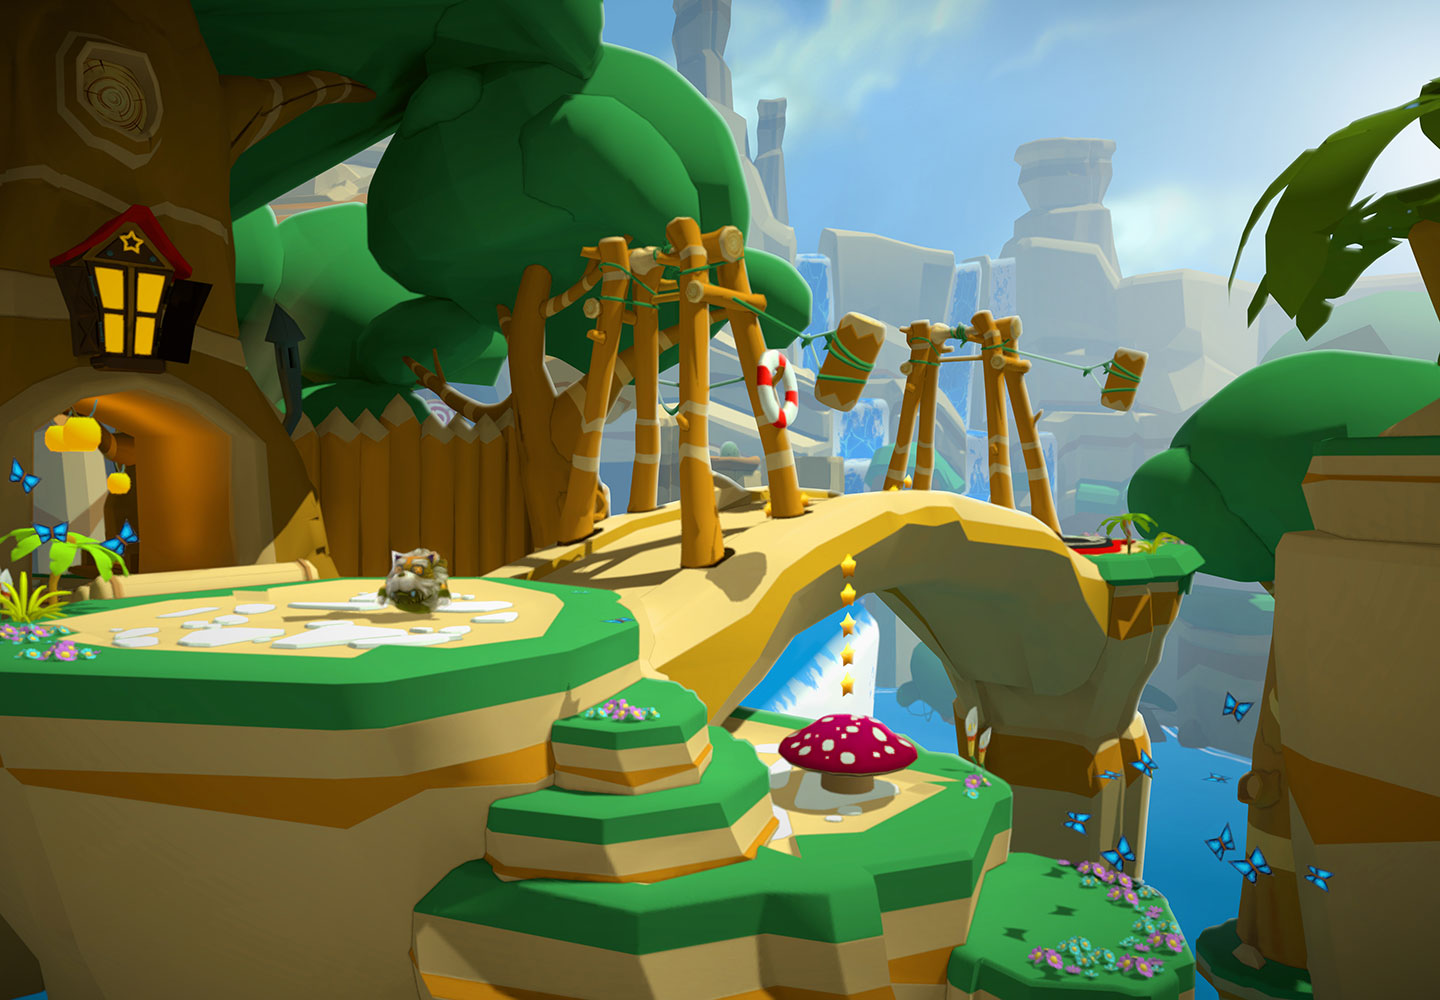
\includegraphics[width=6cm]{images/game.jpg}};
    \node at (11,5) {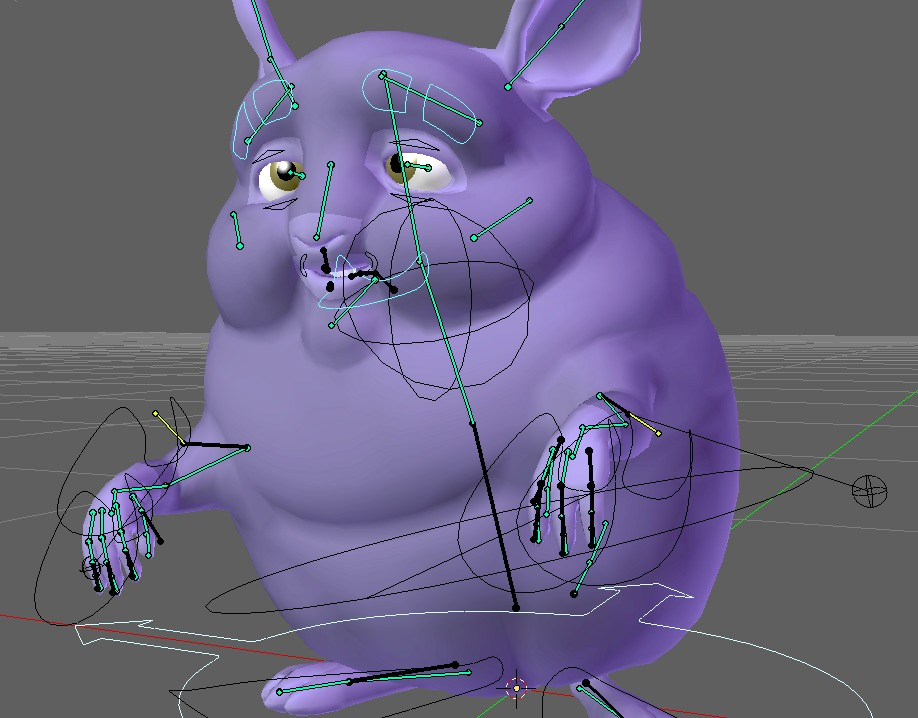
\includegraphics[width=6cm]{images/blender.jpg}};
    \node at (-10,-6) {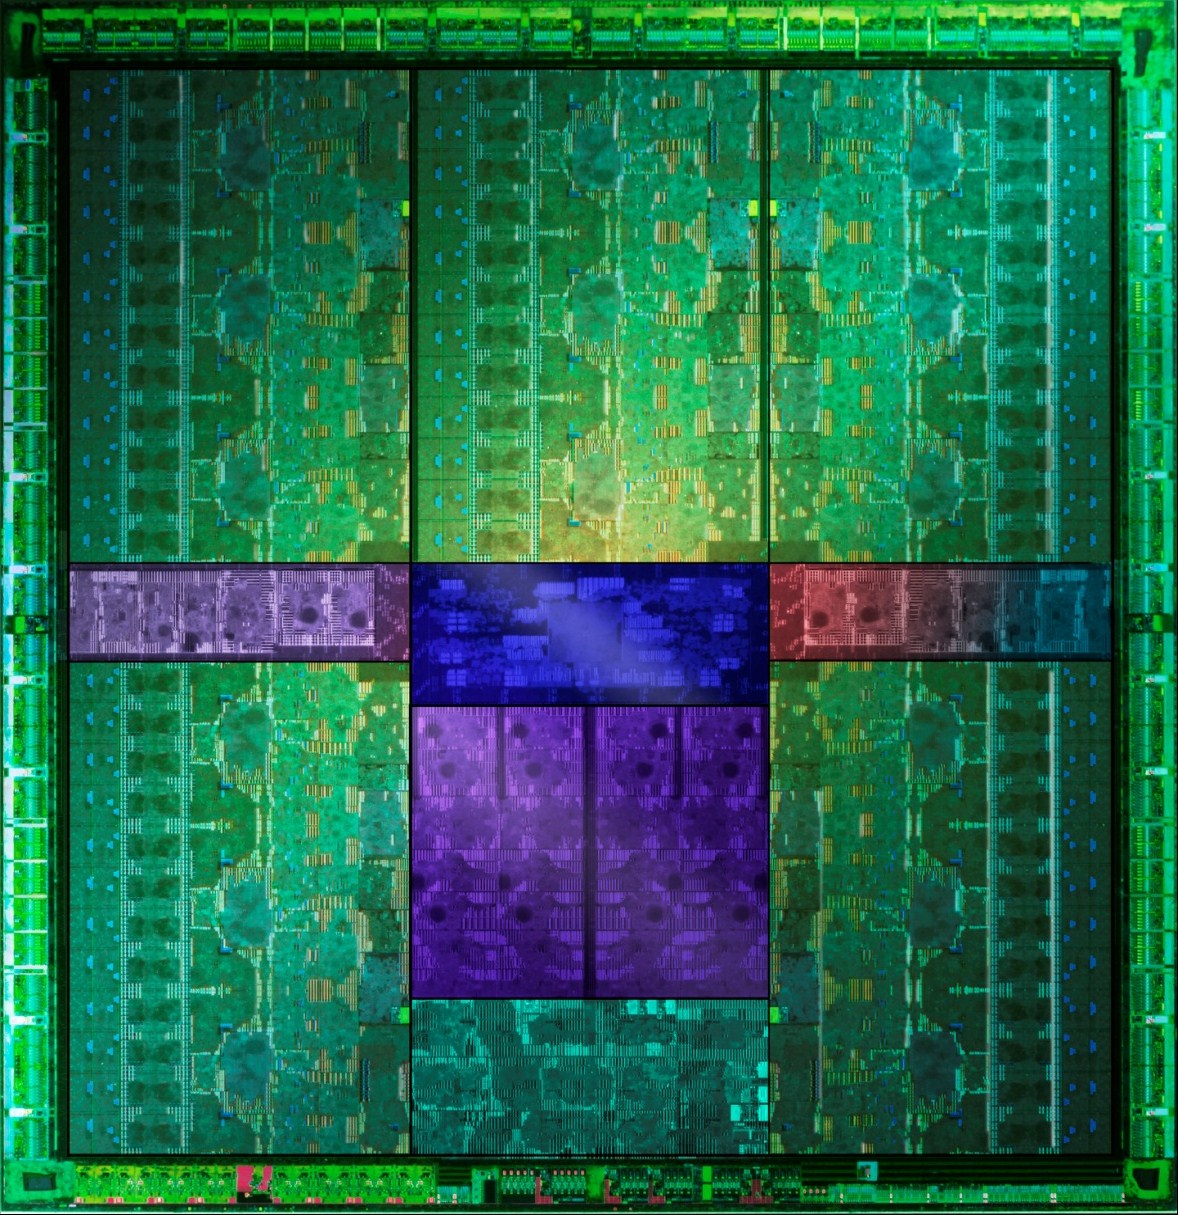
\includegraphics[width=4cm]{images/nvidia-kepler-die.jpg}};
    \begin{scope}[xshift=-0cm, yshift=-12cm,
      base/.style={rectangle, minimum width=10em, minimum height=2em, draw=white, line width=2pt,
        anchor=south west},
      double/.style={base, minimum height=4em},
      small/.style={base, minimum width=4em}]
      % \draw [help lines] grid(3,2);
      \node[base, fill=green!20] at (0,0) {XML Registry};
      \node[base, fill=red!20] at (0,2em) {GL API};
      \node[double, fill=blue!20] at (0,4em) {Wrapper};
      \node[small, fill=green!20] at (-4em,4em) {ctypes};
      \node[small, fill=red!20] at (-4em,6em) {cffi};
      \node[double, minimum width=4em, fill=blue!20] at (-8em,4em) {GL};
      \node[base, fill=green!20] at (0,8em) {High Level API};
    \end{scope}
    \end{tikzpicture}
  \end{center}
}

%%%%%%%%%%%%%%%%%%%%%%%%%%%%%%%%%%%%%%%%%%%%%%%%%%%%%%%%%%%%%%%%%%%%%%%%%%%%%%%%
% Second column
\column{.5}

\block[]{PyDVI\\ a Python library to read and process DVI files}{
  % une bibliothéque Python pour lire et ... des fichiers DVI
  \begin{center}
    \begin{tabular}[t]{p{18cm}p{18cm}}
      \begin{minipage}[t]{17cm}
        \begin{itemize}
        \item DVI $\longrightarrow$ PNG tool
        \item OpenGL Viewer \\
          Font Map Texture \\[.5em]
        
\includegraphics[width=8em]{images/font-map.png}
        \end{itemize}
      \end{minipage}
      & 
      \begin{center}
        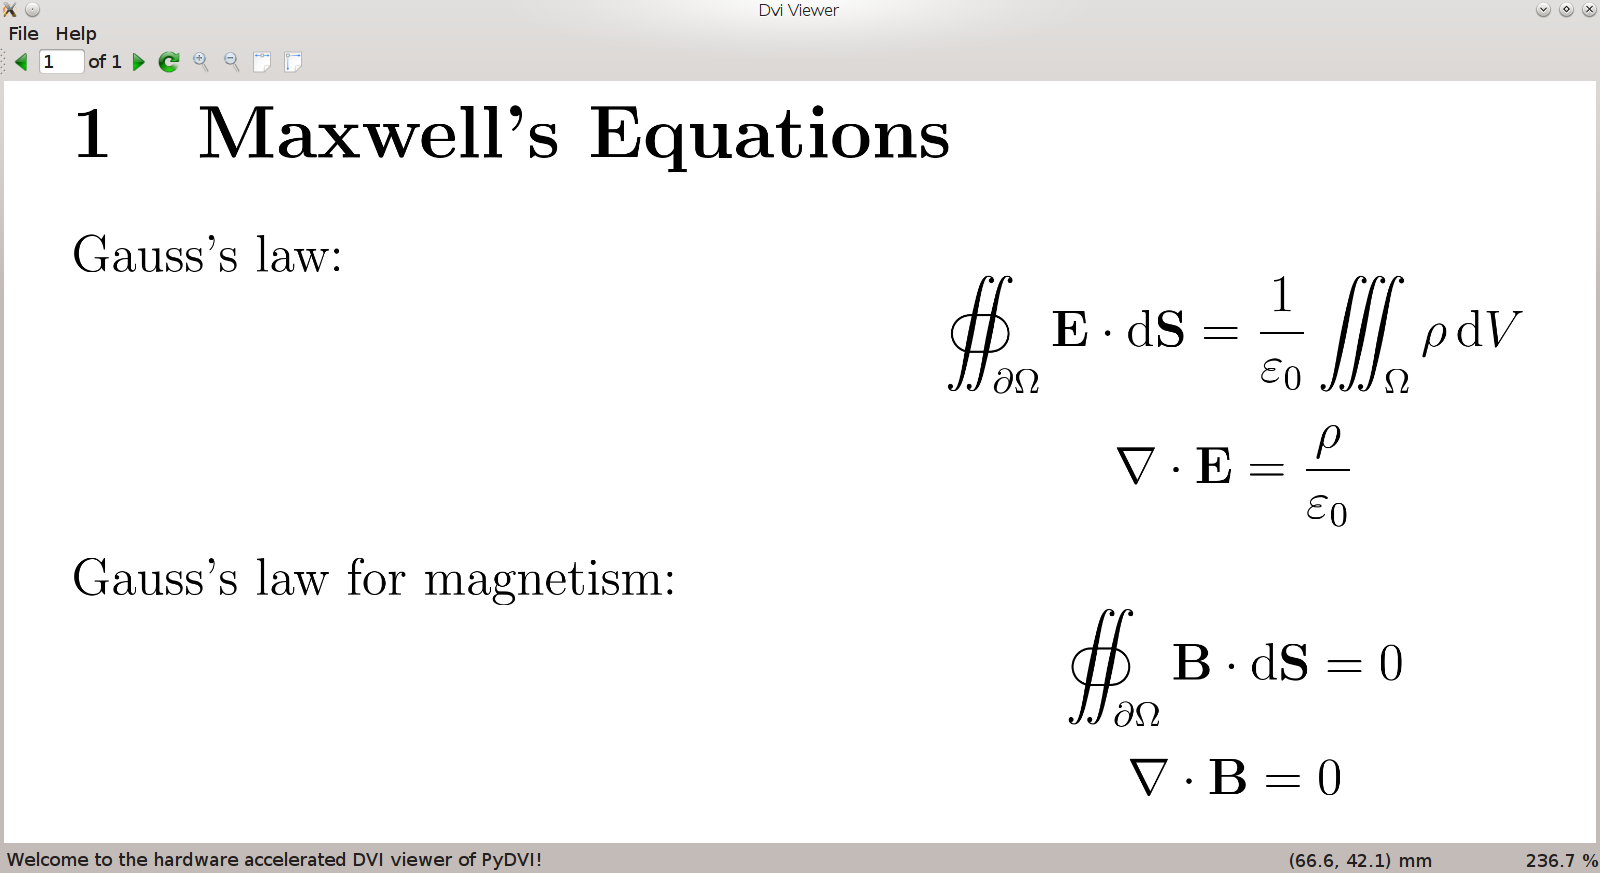
\includegraphics[width=15em]{images/dvi-gl-viewer.png}
      \end{center} \\[1cm]
      \begin{itemize}
      \item packed font, Type 1, virtual font
      \item TeX font metric, Adobe Font Metrics
      \item font map
      \item font encoding
      \end{itemize}
      &
      \begin{center}
        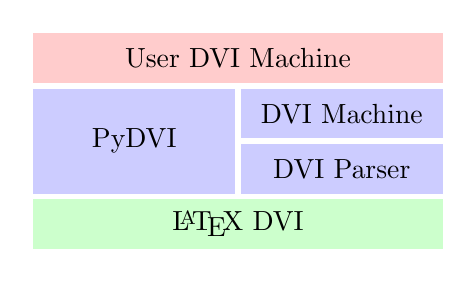
\begin{tikzpicture}[%
          base/.style={rectangle, minimum width=15em, minimum height=2em, draw=white, line width=2pt, anchor=south west},
          demibloc/.style={base, minimum width=7.5em}]
          \node[base, fill=green!20] at (0,0) {\LaTeX{} DVI};
          \node[demibloc, minimum height=4em, fill=blue!20] at (0,2em) {PyDVI};
          \node[demibloc, fill=blue!20] at (7.5em,2em) {DVI Parser};
          \node[demibloc, fill=blue!20] at (7.5em,4em) {DVI Machine};
          \node[base, fill=red!20] at (0,6em) {User DVI Machine};
        \end{tikzpicture}
      \end{center}
    \end{tabular}
  \end{center}
  \begin{flushright}
    https://github.com/FabriceSalvaire/PyDVI
  \end{flushright}
}

\block[titleleft]{Contact: \emailOrange}{%
% \homePageOrange
  
\includegraphics[width=10cm]{figures/vcard.pdf} % check data
}

\end{columns}
\end{document}
\endinput

%%%%%%%%%%%%%%%%%%%%%%%%%%%%%%%%%%%%%%%%%%%%%%%%%%%%%%%%%%%%%%%%%%%%%%%%%%%%%%%%%%%%%%%%%%%%%%%%%%%%%%%%%%%%%%%%%%%%%%%%
%%%
%%% Local Variables: 
%%% mode: latex
%%% TeX-master: t
%%% End: 
%%%
%%%%%%%%%%%%%%%%%%%%%%%%%%%%%%%%%%%%%%%%%%%%%%%%%%%%%%%%%%%%%%%%%%%%%%%%%%%%%%%%%%%%%%%%%%%%%%%%%%%%%%%%%%%%%%%%%%%%%%%%
